\chapter{倫理ある商取引ゲーム}
前章では合理的なプレイヤー達による「商取引ゲーム」において、不正を防止するインセンティブ設計が不可能であることを示した。
しかしながら、現実に住む我々は商取引で必ず不正に合うわけではなく、ある程度は不正が防止されている。
本章では、この理論と現実の差異は限定合理性にあると考え、
そうした戦略をとるプレイヤーのみで構成されたときに不正を防止することができる「倫理ある商取引ゲーム」をモデリングする。
そして、そのモデルが全ての戦略をとりえるプレイヤーによって構成された「商取引ゲーム」においても、
プレイヤーの構成次第で不正を防止するインセンティブ設計として機能することを示す。

\section{本章における問題提起}
前章では商取引ゲームにおいて必ず不正が防止できるようなインセンティブの設計が不可能であることを示した。
しかしながら、現実的に私達は商取引で不正行為に遭遇することは稀である。
なぜ先の理論では商取引で不正を防止するインセンティブ設計ができないにも関わらず、
現実の生活の中で我々は商取引を成功させることができているのだろうか。

\section{本章の仮説}
この問いの答えは、限定合理性(Simon 1947\cite{simon 1947})によって戦略の均衡点が変化し、
不正を防止できるインセンティブ設計が可能になっているためだと思われる。
限定合理性とは、認知能力の限界によって意思決定主体が限られた合理性しか持ち得ないことである。
各プレイヤーにとっての最適な戦略は他のプレイヤーがとる戦略に依存しているため、
当然、一部のプレイヤーが合理的に戦略を選ばないのであれば最適な戦略の均衡点も変化する。
それによって、全てのプレイヤーが合理的である「商取引ゲーム」においては不可能だった
相手が不正を行う可能性を推定することが可能になり、不正を防止するインセンティブ設計が可能になると予想される。

\section{提案手法}
このような限定合理性を「倫理」と呼び、不正行為にあった場合に必ず「失敗」を報告する行動規範とする。
また、この倫理に従うプレイヤーのみによって構成される「商取引ゲーム」を「倫理ある商取引ゲーム」とする。
本章では、「倫理ある商取引ゲーム」において、不正が防止されるインセンティブ設計を行い、
そのインセンティブ設計を通常の「商取引ゲーム」にも適用することで、
プレイヤーの構成によっては不正を防止することが可能になることを示す。

\subsection{倫理ある商取引ゲーム}
「倫理ある商取引ゲーム」とは、$seller$が不正を行った場合に$buyer$がかならず「失敗」を報告する「商取引ゲーム」である。
このゲームのゲーム木と非協力戦略型ゲームの利得は図\ref{ethical-gametree}と表\ref{ethical-gametable}のように表せる。

\subsection{誠実な戦略をとった割合と成功が報告される割合の関係}
「倫理ある商取引ゲーム」においては,全てのプレイヤーは「倫理」に従っているため、
商取引の真の成功率は「商取引システム」に「成功」が報告された割合以上となる。
つまり、任意のプレイヤー$p$と$q$が過去に「商取引ゲーム」を行った際に、
誠実な戦略($s^{seller}_1$もしくは$s^{buyer}_1$)をとってきた割合$HonestStrategyRate(p, q)$と、
成功が報告された割合$ReportedSuccessRate(p, q)$について、次の関係がいえる。

\begin{equation}
  HonestStrategyRate(p, q) \geq ReportedSuccessRate(p, q)
\end{equation}

\section{「倫理ある商取引ゲーム」において不正が防止される条件}
\subsection{不正が抑制される戦略組と期待利得の不等式}
「倫理ある商取引ゲーム」において、不正を防止するためには、
$seller$と$buyer$の戦略組を$(s^{seller}_1, s^{buyer}_1)$に帰着させる必要がある。.
そのためには$seller$が戦略$s^{seller}_1$をとった場合の期待利得$E(r|s^{seller}_1)$が
戦略$s^{seller}_2$をとった場合の期待利得$E(r|s^{seller}_2)$より大きく,
$buyer$が戦略$s^{buyer}_1$をとった場合の期待利得$E(r|s^{buyer}_1)$が
戦略$s^{buyer}_3$をとった場合の期待利得$E(r|s^{buyer}_3)$より大きくならなければならない.
つまりは,$E(r|s^{seller}_1) > E(r|s^{seller}_2)$かつ$E(r|s^{buyer}_1) > E(r|s^{buyer}_3)$を満たす
$(r^{seller}_{success}, r^{seller}_{failure}, r^{buyer}_{success}, r^{buyer}_{failure})$の組を
「商取引システム」から決定できる必要がある.

\subsection{$ seller $と$ buyer $の期待利得}

$ seller $と$ buyer $の各戦略の利得の期待値は以下のように表せる.\\


$ E(R|s^{seller}_1) = p^{buyer}_1 (r^{seller}_{success} + \epsilon^{seller}) + p^{buyer}_3 (r^{seller}_{failure} + \lambda^{seller}) $ \\

$ E(R|s^{seller}_2) = p^{buyer}_1 (goods + r^{seller}_{failure} + \lambda^{seller}) + p^{buyer}_3 (goods + r^{seller}_{failure} + \lambda^{seller}) $ \\

$ = goods + r^{seller}_{failure} + \lambda^{seller} $ \\

$ \because p^{buyer}_1 + p^{buyer}_3 = 1 $(「倫理ある商取引ゲーム」において、$ p^{buyer}_2 $と$ p^{buyer}_4 $は0であるため) \\

$ E(R|s^{buyer}_1) = p^{seller}_1 (goods + r^{buyer}_{success} + \epsilon^{buyer}) + p^{seller}_2 (r^{buyer}_{failure} + \lambda^{buyer}) $ \\

$ E(R|s^{buyer}_3) = p^{seller}_1(goods+r^{buyer}_{failure} + \lambda^{buyer}) + p^{seller}_2 (r^{buyer}_{failure} + \lambda^{buyer}) $ \\

$ = p^{seller}_1 goods + r^{buyer}_{failure} + \lambda^{buyer} $ \\

$ \because p^{seller}_1 + p^{seller}_2 = 1 $ \\


\subsection{$ seller $が誠実な戦略をとる条件}

$ E(R|s^{seller}_1) > E(R|s^{seller}_2) $ \\

$ \therefore p^{buyer}_1 (r^{seller}_{success} + \epsilon) + p^{buyer}_2 (r^{seller}_{failure} + \lambda) > goods + r^{seller}_{failure} + \lambda $ \\

$ \therefore p^{buyer}_1(r^{seller}_{success} + \epsilon) - p^{buyer}_1(r^{seller}_{failure} + \lambda) > goods $ \\

$ \therefore p^{buyer}_1(r^{seller}_{success} - r^{seller}_{failure} + \epsilon - \lambda) > goods $ \\

仮定より,$ \epsilon > \lambda $のため,
$ p^{buyer}_1 (r^{seller}_{success} - r^{seller}_{failure}) \geq goods $を満たせばよい.

$ 0 < p^{buyer}_1 $を仮定するならば,
$ r^{seller}_{success} - r^{seller}_{failure} \geq \frac{goods}{p^{buyer}_1} $


\subsection{$ buyer $が誠実な戦略をとる条件}

$ E(R|s^{buyer}_1) > E(R|s^{buyer}_3) $ \\

$ \therefore p^{seller}_1 (goods + r^{buyer}_{success}) + p^{seller}_2 r^{buyer}_{failure} > p^{seller}_1(goods+r^{buyer}_{failure}) + p^{seller}_2 r^{buyer}_{failure} $ \\

$ \therefore p^{seller}_1(r^{buyer}_{success} - r^{buyer}_{failure}) > 0 $ \\

$ 0 < p^{seller}_1 $を仮定するならば, \\

$ r^{buyer}_{success} - r^{buyer}_{failure} > 0 $ \\

上記をまとめると,$ 0<p^{buyer}_1 $かつ $ 0 < p^{seller}_{1} $を仮定した上で,\\

$ r^{seller}_{success} - r^{seller}_{failure} \geq \frac{goods}{p^{buyer}_1} $かつ$ r^{buyer}_{success} - r^{buyer}_{failure} > 0 $ \\

を満たせば,「倫理ある商取引ゲーム」で不正を防止することができる.


\subsection{信頼度 $ p^{player} $}

ここで,任意の$ player $が誠実な戦略($ p^{seller}_1, p^{buyer}_1 $のいづれか)をとる主観確率を$ p^{player}_1 $とすると,
$ p^{player}_1 $は各プレイヤーに対して誠実な戦略をとった割合$ HonestyStrategyRate(player, opportunity) $と任意の重み$ w^{player} $を用いて次のように表せる. \\

\begin{equation}
  p^{player}_1 \equiv \sum^{players}_{opp} w^{opp} HonestyStrategyRate(player, opp)
\end{equation}

\subsection{最低信頼度 $ T^{player} $}

しかし、「商取引システム」からは$ HonestyStrategyRate(player, opportunity) $は未知のため,
信頼度$ p^{player}_1 $を求めることができない.
そこで$ HonestyStrategyRate $の代わりに$ ReportedSuccessRate $を用い、
信頼度$ p^{player} $を計算するのと同じ重み$ w^{player} $の荷重総和をとったものを、
最低信頼度$ T^{player} $と定義する. \\

\begin{equation}
  T^{player} \equiv \sum^{players}_{opp} {w}^{opp} ReportedSuccessRate(player, opp)
\end{equation}

\subsection{最低信頼度を用いた条件}
ここで$ HonestyStrategyRate \geq ReportedSuccessRate $であるため,$ p^{player}_1 \geq T^{player} $がいえる.

ゆえに, \\

\begin{equation}
  r^{seller}_{success} - r^{seller}_{failure}  \geq \frac{goods}{T^{buyer}} \geq \frac{goods}{p^{buyer}_1}
\end{equation}

となる.

つまり、$ 0<p^{buyer}_1 $かつ $ 0 < p^{seller}_{1} $を仮定した上で,\\

\begin{equation}
  r^{seller}_{success} - r^{seller}_{failure} \geq \frac{goods}{T^{buyer}} かつ r^{buyer}_{success} - r^{buyer}_{failure} > 0
\end{equation}

を満たす$ (r^{seller}_{success}, r^{seller}_{failure}, r^{buyer}_{success}, r^{buyer}_{failure}) $の組を「商取引システム」から決定できれば、
「倫理ある商取引ゲーム」において不正を防止することができる。

\section{実験方法}
先の不正が防止される条件を満たすインセンティブ設計を行う「商取引システム」と
次の8タイプのエージェントから重複問わずランダムに選んだ8体のエージェントを用意し試行を実施する。
これを、タイプAのエージェントが0~7体を占める場合について8000回づつ繰り返し、
エージェントの構成とstep13で求まる「報告された成功率」と「真の成功率」を記録する。

\subsection{エージェントの種類}
下記の8タイプのエージェントを用意する。
\begin{itemize}
  \item [Type A] sellerのとき商品を送り、buyerのときは商品を受け取った場合は「成功」、受け取らなかった場合は「失敗」を報告する。
  \item [Type B] sellerのとき商品を送り、buyerのときは商品を受け取った場合は「成功」、受け取らなかった場合は「成功」を報告する。
  \item [Type C] sellerのとき商品を送り、buyerのときは商品を受け取った場合は「失敗」、受け取らなかった場合は「成功」を報告する。
  \item [Type D] sellerのとき商品を送り、buyerのときは商品を受け取った場合は「失敗」、受け取らなかった場合は「失敗」を報告する。
  \item [Type E] sellerのとき商品を送らず、buyerのときは商品を受け取った場合は「成功」、受け取らなかった場合は「失敗」を報告する。
  \item [Type F] sellerのとき商品を送らず、buyerのときは商品を受け取った場合は「成功」、受け取らなかった場合は「成功」を報告する。
  \item [Type G] sellerのとき商品を送らず、buyerのときは商品を受け取った場合は「失敗」、受け取らなかった場合は「成功」を報告する。
  \item [Type H] sellerのとき商品を送らず、buyerのときは商品を受け取った場合は「失敗」、受け取らなかった場合は「失敗」を報告する。
\end{itemize}

\subsection{試行}
\begin{itemize}
  \item[step 1] 時刻tを0とする。
  \item[step 2] 「商取引システム」の各エージェントの通貨保有量を8とする。
  \item[step 3] 各プレイヤーが互いにsellerとbuyerのそれぞれの役割で1度づつ商取引ゲームを行う順序を決定する。(順序の長さは56となる)
  \item[step 4] 時刻tを1進める。
  \item[step 5] step 3で決定した順序を周期として、sellerとbuyerを決定する。
  \item[step 6] 「商取引システム」はこれまで報告された結果から、「成功」と「失敗」が報告された場合のsellerとbuyerの通貨保有量を計算する。
  \item[step 7] sellerは自身の戦略に基づいて、buyerに商品を送るか、もしくは商品を送らない。
  \item[step 8] buyerは自身の戦略とstep 6のsellerの行動に基づいて、「商取引ゲーム」 の結果を決定する。
  \item[step 9] buyerは決定した結果を「商取引システム」に報告する。 
  \item[step 10] 「商取引システム」はstep6で計算した通貨保有量がいずれの場合にも0未満にならない場合、 buyerから報告された結果を記録する。
  \item[step 11] step6で計算した通貨保有量がいずれの場合にも0未満にならない場合、真の結果を記録する。
  \item[step 12] 時刻tが1120未満なら、step4に戻る。
  \item[step 13] 過去56回の商取引ゲームにおいて、step10と11で記録された結果を集計し、それぞれ「報告された成功率」と「真の成功率」を求める。
\end{itemize}

\section{「商取引システム」の詳細}
本節ではシミュレーションに用いる「評判システム」の仕様の詳細を紹介する。
完全な実装については、GitHubのソースコードを参照。

\subsection{約束の価値$C$}
\begin{eqnarray}
  C &\equiv& 1 \\
    &=& c_{p2} - c_{p1} \\
    &=& c_{r1} - c_{r2}
\end{eqnarray}

\subsection{ReputationWeight}
最低信頼度$ T_i $を求めるため、$ReportedSuccessRate(i, j)$の荷重総和に用いる重み$ w_k $を定義する.
この重み$w_k$は、任意の成員$i$が戦略$s_{p1}$をとる確率$p_{p1}$を推定する際に、
成員$i$と他の成員$j$における$ReportedSuccessRate(i, j)$をどの程度信頼するかを表している。
本実験では、成員$j$の「評判スコア」が全体に占める割合をReputationWeight$w_j$と定義する。
任意の成員$k$の「評判スコア」を$b_k$としたとき、$w_k$は次のように表せる。($n$は成員の人数)

\begin{equation*}
  w_k \equiv \frac{b_k}{\sum^{\{1,2,...,n\}}_{k}b_k}
\end{equation*}

\subsection{「成功」が報告された場合の「評判スコア」の変化}
$ reporter $が「成功」を報告した場合、
$ reporter $は約束の価値$C$だけ減り、$ promisor $は$C$だけ増加するものとする。

\begin{gather}
  r_{ps} = C \\
  r_{rs} = -C \\
  r_{ps} + r_{rs} = 0
\end{gather}


\subsection{EscrowCost}
「失敗」が報告されたとき、$promisor$と$reporter$が失う「評判スコア」の合計を$EscrowCost$とする。
約束の価値$C$にエスクロー係数$E$を掛けたものとする.

\begin{eqnarray}
  EscrowCost  &\equiv& (r_{rs} - r_{rf}) + (r_{ps} - r_{pf}) \\
              &=& E \cdot C \label{escrowCost}
\end{eqnarray}

\subsection{EscrowCostの負担比率}
成員$i$を$promiser$、$j$を$reporter$とする。
「約束・評判ゲーム」を行うとき、$EscrowCost$の負担比率を両者の最低信頼度$T_i$を用いる.\\

\begin{equation}
  (r_{ps} - r_{pf}):(r_{rs} - r_{rf}) = T_j:T_i
\end{equation}

\subsection{EscrowCostの分配}
「失敗」が報告されたときに$EscrowCost$が消失すると、
「評判スコア」の総量が下がり、約束の価値$C$

総量を一定に保つために、$promisor$と$reporter$以外の全てのプレイヤーに、
$ReputationWeight$に応じて$EscrowCost$を分配する。
$promisor$と$reporter$を含まないのは、分配によるインセンティブ設計への影響をなくすためである。

\subsection{不正が防止される条件を満たす定義}
成員$j$を$promiser$、$k$を$reporter$とする。
このとき、\eqref{condition6-1}と\eqref{condition6-2}を満たす$r_{ps} - r_{pf}$と$r_{rs} - r_{rf}$を下記のように定義する。

\begin{eqnarray}
  r_{ps} - r_{pf} &\equiv& \frac{C}{T_i} \label{condition6-3} \\
                  &\geq& \frac{c_{p2} - c_{p1}}{T_i} \nonumber \\
  r_{rs} - r_{rf} &\equiv& \frac{C}{T_j} \label{condition6-4} \\
                  &\geq& 0 \nonumber
\end{eqnarray}

\subsection{残高の変化量の組$ (r_{ps}, r_{pf}, r_{rs}, r_{rf}) $}
上記の定義からエスクロー係数$E$と残高の変化量の組$ (r_{ps}, r_{pf}, r_{rs}, r_{rf}) $は次のように求まる. \\
成員$i$を$promisor$、$j$を$reporter$とする。

\begin{eqnarray}
  E &=& - \frac{T_i + T_j}{T_i T_j} \\
  r_{ps} &=& 1 \\
  r_{pf} &=& 1 - \frac{1}{T_j} \\
  r_{rs} &=& -1 \\
  r_{rf} &=& -1 - \frac{1}{T_i}
\end{eqnarray}


\section{評価}
先の実験の結果、「報告された成功率」と「真の成功率」の両方が100\%になった場合を「不正防止の成功」とし、
誠実なエージェント(タイプA)の数と「不正防止の成功」に至った割合をプロットしたものが、図\ref{ethical-game-001}である。
(エージェント数8の場合は、エージェントの組み合わせが1通りしか存在しないため、個別に試行を行い結果を集計している。)
誠実なエージェントの数が0体の場合であっても不正が防止される構成が存在し、
6体以上の場合はサンプリングした全ての構成で不正の防止が成功していた。

\begin{figure}[h]
  \begin{tabular}{cc}
    \begin{minipage}[t]{1\hsize}
      \centering
      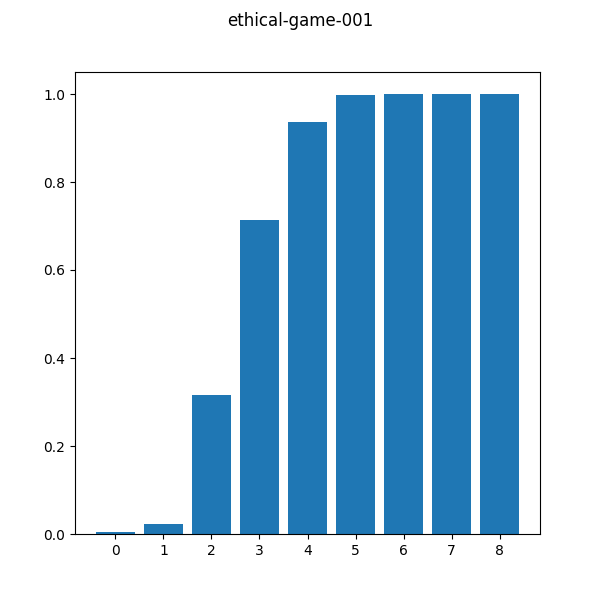
\includegraphics[keepaspectratio, width=1\linewidth]{./04_ethical-commerce-game/ethical-game-001.png}
      \caption{誠実なエージェントの数と「不正防止の成功」に至った割合}
      \label{ethical-game-001}
    \end{minipage}
  \end{tabular}
\end{figure}

\section{結論}
実験とその評価を踏まえて、「倫理」という限定合理性を仮定した上でインセンティブ設計を行うことで、
プレイヤーの構成によっては「商取引ゲーム」において不正を防止することが可能であることがわかる。
また、プレイヤーの構成と不正防止の成功成功の関係性については、先の実験の図のとおりである。

\clearpage
\begin{figure*}
  \centering
  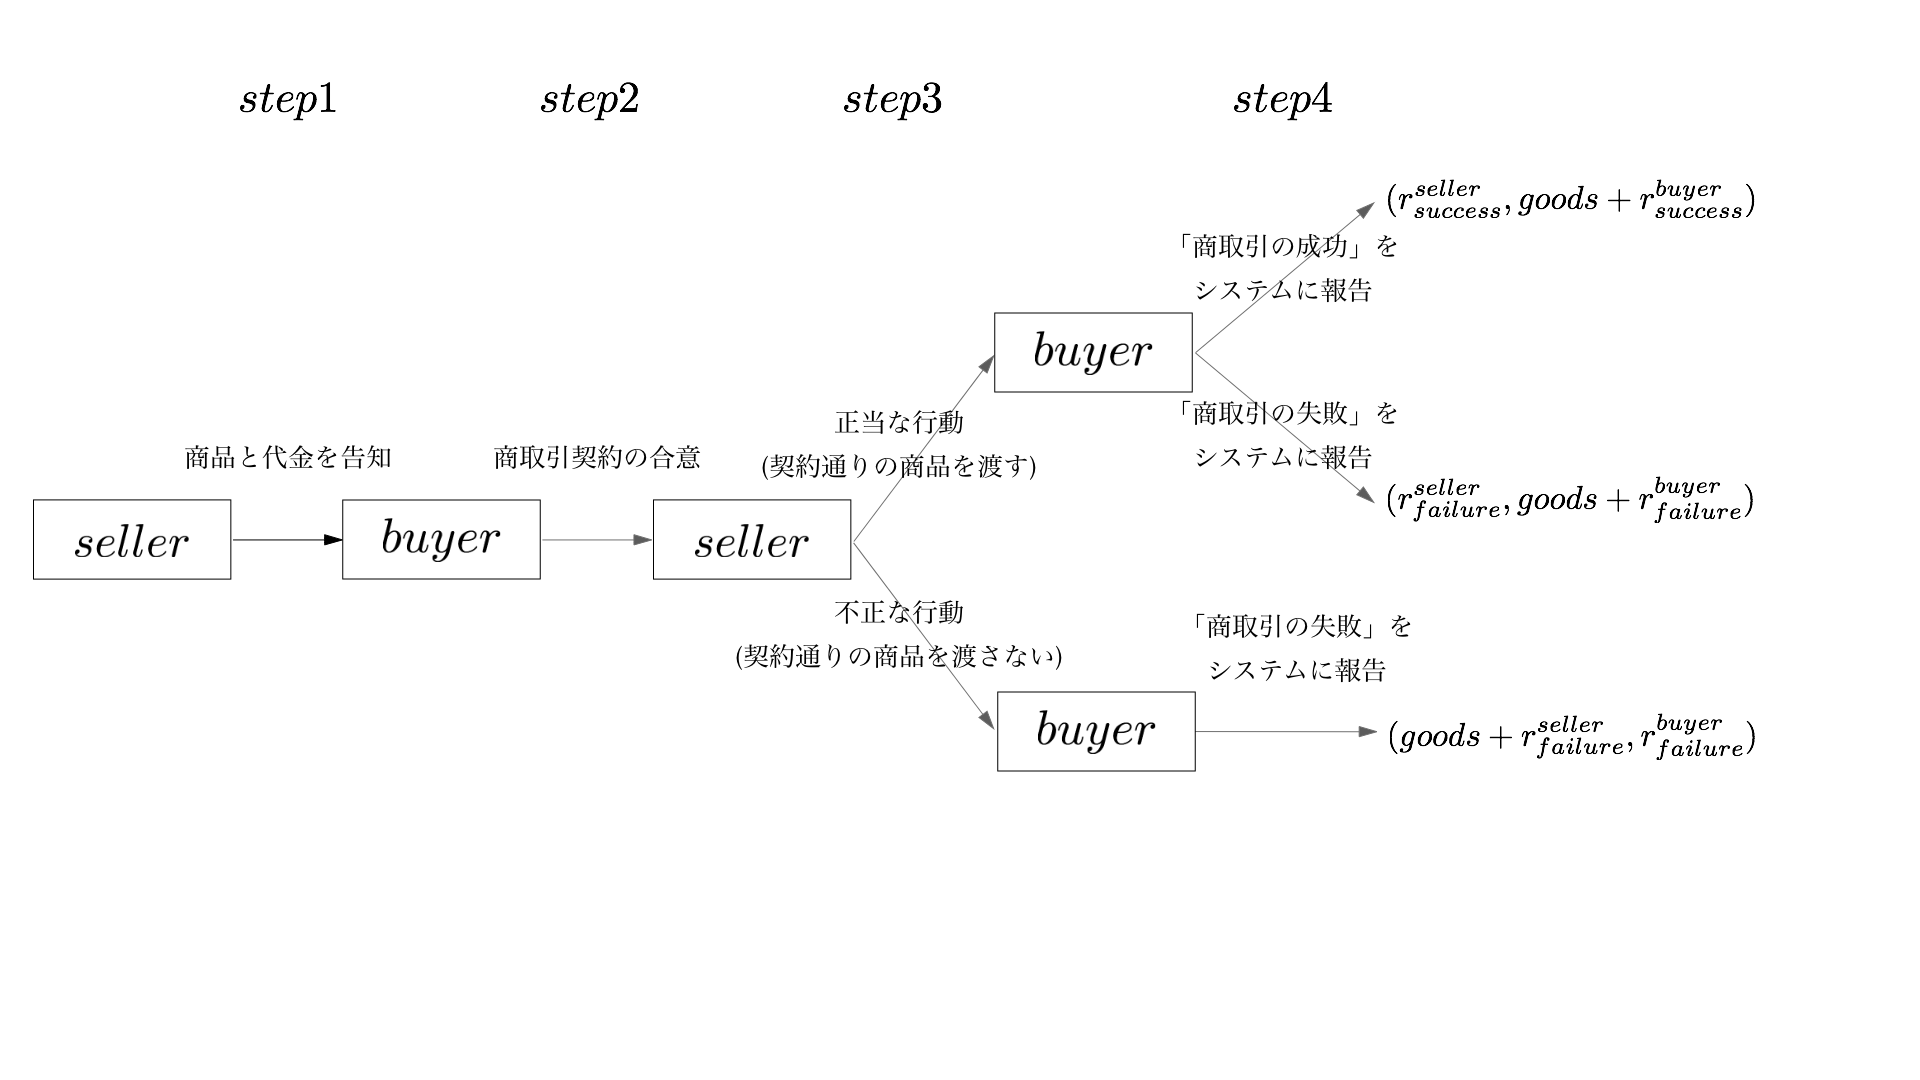
\includegraphics[width=1\linewidth]{./06_ethical-commerce-game/ethical-gametree.png}
  \caption{「倫理ある商取引ゲーム」のゲーム木}
  \label{ethical-gametree}
\end{figure*}

\subsection{非協力戦略型ゲーム}
\newcommand{\successseller}{
  \begin{tabular}{c}
    $(r^{seller}_{success},$\\
    $goods+r^{buyer}_{success})$
  \end{tabular}
}
\newcommand{\successbuyer}{
  \begin{tabular}{c}
    $(goods+r^{seller}_{success},$\\
    $r^{buyer}_{success})$
  \end{tabular}
}
\newcommand{\fseller}{
  \begin{tabular}{c}
    $(r^{seller}_{failure},$\\
    $goods+r^{buyer}_{failure})$
  \end{tabular}
}
\newcommand{\fbuyer}{
  \begin{tabular}{c}
    $(goods+r^{seller}_{failure},$\\
    $r^{buyer}_{failure})$
  \end{tabular}
}

\begin{table*}
  \centering
  \begin{tabular}{|l|l|l|l|}
    \hline
    \multicolumn{2}{|l|}{\multirow{2}{*}{}} & \multicolumn{2}{l|}{$buyer$} \\ \cline{3-4}
    \multicolumn{2}{|l|}{}                  &$s^{buyer}_1$&$s^{buyer}_3$\\ \hline
    \multirow{2}{*}{$seller$}
    &$s^{seller}_1$&\successseller&\fseller\\ \cline{2-4}
    &$s^{seller}_2$&\fbuyer&\fbuyer\\ \hline
  \end{tabular}
  \caption{非協力戦略型ゲームとして表した「倫理ある商取引ゲーム」の利得表}
  \label{ethical-gametable}
\end{table*}

% 倫理ある商取引ゲーム
% \section{倫理ある商取引システムの詳細}
「倫理ある商取引ゲーム」においては,最低信頼度$ T^{player} $を用いた上記の条件式を満たせば,不正を防止することが可能になる.ただ,上記の条件のみでは「商取引システム」から保有通貨の変化量の組$ (r^{seller}_{success}, r^{seller}_{failure}, r^{buyer}_{success}, r^{buyer}_{failure}) $を一意に決定できないので,いくつかの条件を追加する.


\subsection{取引成功前後の残高の変化}
商取引成功前後では$ buyer $は商品$ goods $の価格$ price $だけ残高が減り$ seller $は$ price $だけ残高が増えるものとする.そのため商取引前後では$ seller $と$ buyer $の残高の合計は変化しない.ここから,$ r^{seller}_{success} $と$ r^{buyer}_{success} $は以下のように記せる.

$ r^{seller}_{success} = price $
$ r^{buyer}_{success} = -price $
$ r^{seller}_{success} + r^{buyer}_{succcess} = 0 $

\subsection{エスクロー係数 E}
まずは「失敗」が報告された時に$ seller $と$ buyer $から失われる通貨の量の合計を$ EscrowCost $とおいて考え,同時に商品価格$ price $にエスクロー係数$ E $を掛けたものとする.(ここで$ price $は$ goods $の価格である)

$ EscrowCost \equiv (r^{buyer}_{success} - r^{buyer}_{failure}) + (r^{seller}_{success} - r^{seller}_{failure}) $
$ = E \cdot price $

\subsection{負担比率}
ここで問題となるのは$ EscrowCost $を求めるための$ seller $と$ buyer $の負担比率をどのようにして決定するかである.本稿では最低信頼度$ T^{player} $を用いてこの負担比率を決定することとする.

$ (r^{buyer}_{success} - r^{buyer}_{failure}):(r^{seller}_{success} - r^{seller}_{failure}) = w(T^{buyer}):w(T^{seller}) $

ここで最低信頼度が高い$ player $の方が負担比率が小さくなるように責任比重関数$ w(x) $は値域$ 0 \leq  x \leq 1 $において$ w'(x)>0 $を満たすものとする.

\subsection{責任比重関数$ w(x) $}
本稿では負担比重関数は恒等写像$ w(x)=x $とする.

\subsection{ReputationWeights}
最低信頼度$ T^{player} $を求めるにあたって$ r.w.^{opportunity} $を決定する必要がある.$ r.w.^{opportunity} $は誠実さ$ T^{player}_1 $を求める際に$ ReportedSuccessRate(player, opportunity) $に係る任意の重みである.これはつまり任意の$ player $が誠実な戦略をとる主観的確率を考える際に,$ player $と$ opportunity $の間であった過去の商取引での報告された成功率をどの程度信じるかである.仮に$ player $と$ opportunity $の間で信頼関係があれば$ ReportedSuccessRate $は$ 1 $になる.なので「商取引システム」の参加者数$ n $が特定できる場合は$ \frac{1}{n} $が妥当だろう.逆に不特定多数であり,同一の意志によって複数のプレイヤーが動いている場合は,保有している通貨量$ b^{opportunity} $の全体の通貨の総量に占める割合が良いだろう.

$ r.w.^{opportunity} \equiv \frac{b^{opportunity}}{\sum^{players}_{i}b^{i}} $


\subsection{EscrowCostの分配}
「失敗」が報告されたときに失われる$ EscrowCost $は消滅するのではなく参加者に分配する.これは全体の通貨量の減少によって通貨の価値が上がって商品価格が下がるという経済原理が生じ,インセンティブ設計が複雑化するのを防ぐためである.そこで$ EscrowCost $として失われた通貨は任意の重み$ e.w.^{player} (\sum^{players}_{player}e.w.^{player} = 1) $を用いて分配し「商取引ゲーム」の前後で全体の通貨量を等しくする.

\subsection{EscrowWeights}
EscrowCostの分配に関しては「商取引システム」に参加している各プレイヤーの通貨の保有率に応じて分配する.$ seller $と$ buyer $を含んでいるのは,仮に$ seller $と$ buyer $以外のすべてのプレイヤーで分配した場合,$ seller $もしくは$ buyer $は結託する別のプレイヤーに保有する通貨の一部を一時的に預けることで,その分だけ$ EscrowCost $の負担を軽減することが可能になるためである.そこで本稿では任意の重み$ e.w.^{player} $を以下のように定義する.

$ e.w.^{player} \equiv \frac{b^{player}}{\sum^{players}_{escrow}b^{escrow}} $

\subsection{謎の条件}
$ \frac{w(T^{buyer}_1)E \cdot price}{w(T^{buyer}_1) + w(T^{seller}_1)} \geq \frac{price}{T^{buyer}} \geq \frac{goods}{p^{buyer}_1} $

上記の条件式から$ \frac{price}{ T^{buyer} } $でうまくいくはずだったが何故かうまく行かず,$ \frac{price}{ \min(T^{buyer}, T^{seller})} $をもちいたらうまくいったのでこちらを採用することとした.$ p^{buyer} $と$ P^{player}_1 $の関係性に問題があるためだと思われる.

$ \frac{w(T^{buyer}_1)E \cdot price}{w(T^{buyer}_1) + w(T^{seller}_1)} \geq \frac{price}{ \min(T^{buyer}, T^{seller})} $


\subsection{残高の変化量の組$ (r^{seller}_{success}, r^{seller}_{failure}, r^{buyer}_{success}, r^{buyer}_{failure}) $}
上記の条件群を用いて残高の変化量の組$ (r^{seller}_{success}, r^{seller}_{failure}, r^{buyer}_{success}, r^{buyer}_{failure}) $を決定する.


$ r^{seller}_{success}+r^{buyer}_{success} = 0 $

$ r^{seller}_{failure}+r^{buyer}_{failure} = -E \cdot price $

$ r^{seller}_{success} - r^{seller}_{failure} = \frac{w(T^{buyer}_1)E \cdot price}{w(T^{buyer}_1) + w(T^{seller}_1)} \geq \frac{price}{T^{buyer}} $

$ r^{buyer}_{success} - r^{buyer}_{failure} = \frac{w(T^{seller}_1)E \cdot price}{w(T^{buyer}_1) + w(T^{seller}_1)} \geq 0 $

$ \frac{w(T^{buyer})E \cdot price}{w(T^{buyer}) + w(T^{seller})} = \frac{price}{\min(T^{buyer}, T^{seller})} $

$ E $ = $ \frac{w(T^{buyer})+w(T^{seller})}{w(T^{buyer}) \cdot \min(T^{buyer}, T^{seller})} $

$ r^{seller}_{success}-r^{seller}_{failure} = \frac{price}{min(T^{buyer}, T^{seller})} $

$ r^{buyer}_{success} - r^{buyer}_{failure} = \frac{w(T^{seller}) \cdot price}{w(T^{buyer}) \cdot \min(T^{buyer}, T^{seller})} $


$ r^{seller}_{success} = price $
$ r^{buyer}_{success} = -price $
$ r^{seller}_{failure} = price \cdot (1 - \frac{1}{min(T^{buyer}, T^{seller})}) $
$ r^{buyer}_{failure} = - price \cdot (\frac{T^{seller}}{T^{buyer} \cdot \min(T^{buyer}, T^{seller})} + 1) $
